\documentclass[10pt]{beamer}

\usetheme[progressbar=frametitle]{metropolis}
\usepackage{appendixnumberbeamer}

\usepackage{booktabs}
\usepackage[scale=2]{ccicons}

\usepackage{pgfplots}
\usepgfplotslibrary{dateplot}

\usepackage{subcaption}

\usepackage{graphicx}
\newcommand\scalemath[2]{\scalebox{#1}{\mbox{\ensuremath{\displaystyle #2}}}}

\usepackage{xspace}
\newcommand{\themename}{\textbf{\textsc{metropolis}}\xspace}


\setbeamercolor{alerted text}{fg=teal}
\setbeamercolor{emph}{fg=teal}
\renewcommand<>{\emph}[1]{%
  {\usebeamercolor[fg]{emph}\only#2{\itshape}#1}%
}

\title{An Introduction to Quantum Computers\\ and Hidden Subgroup Problems}
\subtitle{Postquantum Cryptography Reading Group}
% \date{\today}
\date{}
\author{Luke Mader}
% \institute{Lancaster University}

\usepackage[export]{adjustbox}
\usepackage{amsmath,
            amssymb,
            gensymb,
            mathtools
            }

\usepackage{textcomp} % i forget this package's purpose

% \usepackage{pgfplots}
% \pgfplotsset{width=10cm}
\linespread{1.8}


\usepackage{amsthm}

\newcommand{\set}[1]{\left\{#1\right\}}
\newcommand{\N}{\mathbb{N}}
\newcommand{\R}{\mathbb{R}}
\newcommand{\Z}{\mathbb{Z}}
\newcommand{\Q}{\mathbb{Q}}
\newcommand{\C}{\mathbb{C}}
\newcommand{\M}{\mathrm{M}}
\newcommand{\F}{\mathbb{F}}
\newcommand{\HS}{\mathcal{H}}

\newcommand{\eps}{\varepsilon}
\newcommand{\id}{\text{id}}
\newcommand{\dist}[1]{\text{dist}\left(#1\right)}
\newcommand{\ip}[1]{\left\langle #1\right\rangle}
\newcommand{\conjugate}[1]{\mkern 1.5mu\overline{\mkern-1.5mu#1\mkern-1.5mu}\mkern 1.5mu} 
\newcommand{\dom}[1]{\mathrm{Dom}\left(#1\right)}


\DeclarePairedDelimiter\abs{\lvert}{\rvert}%
\DeclarePairedDelimiter\norm{\lVert}{\rVert}%

% Swap the definition of \abs* and \norm*, so that \abs
% and \norm resizes the size of the brackets, and the
% starred version does not.
\makeatletter
\let\oldabs\abs
\def\abs{\@ifstar{\oldabs}{\oldabs*}}
%
\let\oldnorm\norm
\def\norm{\@ifstar{\oldnorm}{\oldnorm*}}
\makeatother


\newcommand{\op}[1]{\norm{#1}_\text{op}}



% bra-ket notation
% uses package mathtools
\DeclarePairedDelimiter\bra{\langle}{\rvert}
\DeclarePairedDelimiter\ket{\lvert}{\rangle}
\DeclarePairedDelimiterX\braket[2]{\langle}{\rangle}{#1 \vert #2}
\DeclarePairedDelimiterX\ketbra[2]{\delimsize\vert}{\delimsize\vert}{#1 \rangle\langle #2}





\newcommand*{\rvec}[1]{\left( #1\right)}
\newcommand*{\tr}[1]{\operatorname{tr}\left(#1\right)}
\newcommand*{\range}[1]{\operatorname{range}\left(#1\right)}
\renewcommand*{\ker}[1]{\operatorname{ker}\left(#1\right)}


\begin{document}
\metroset{block=fill}
\maketitle

\begin{frame}{The plan}
    \begin{enumerate}
        \item An overview of quantum for quantum computing
        % \vspace{1cm}
        \item Some quantum algorithms:\begin{itemize}
          \item The Deutsch problem and phase kickback 
          \item Quantum Fourier transforms and the Deutsch-Jozsa problem 
          \item Simon's problem 
          \item Shor's algorithm
        \end{itemize}
        % \vspace{1cm}
        \item Hidden subgroup problems on finite Abelian groups
    \end{enumerate}
\end{frame}

\begin{frame}{Some good resources}
  \begin{figure}[H]
    This presentation is heavily taken from:

    \bigskip 


    \centering
    \begin{subfigure}{.5\textwidth}
      \centering
      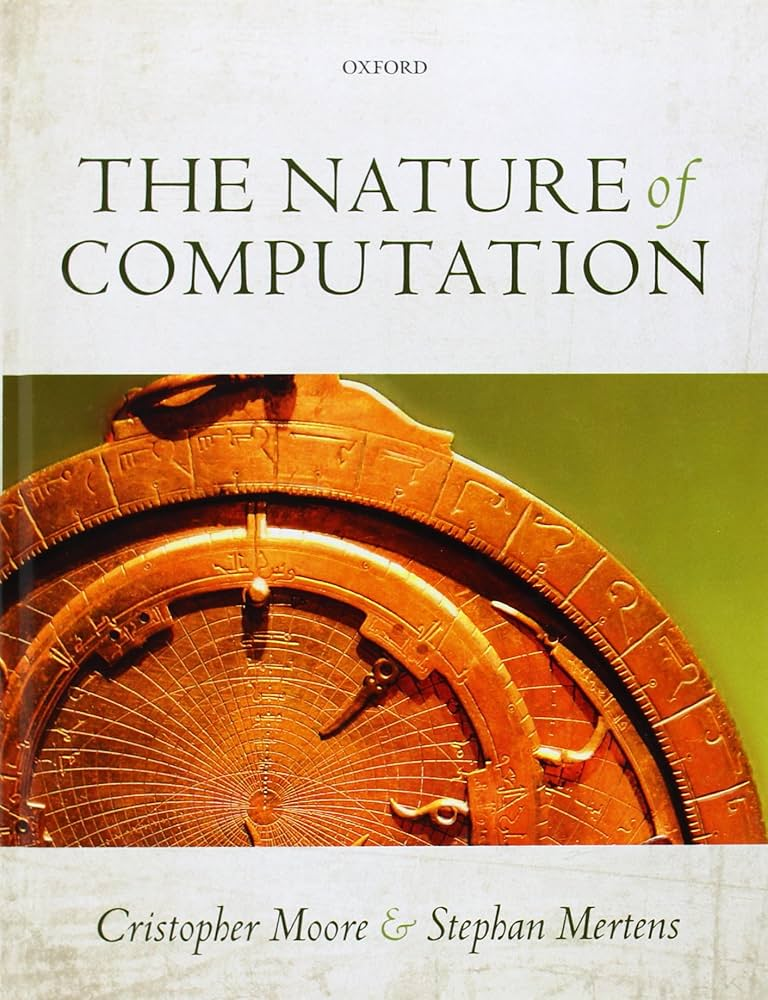
\includegraphics[width=.8\linewidth]{cover_nature_of_computing.jpg}
      \caption{Chapter 15}
      % \label{fig:sub1}
    \end{subfigure}%
    \begin{subfigure}{.5\textwidth}
      \centering
      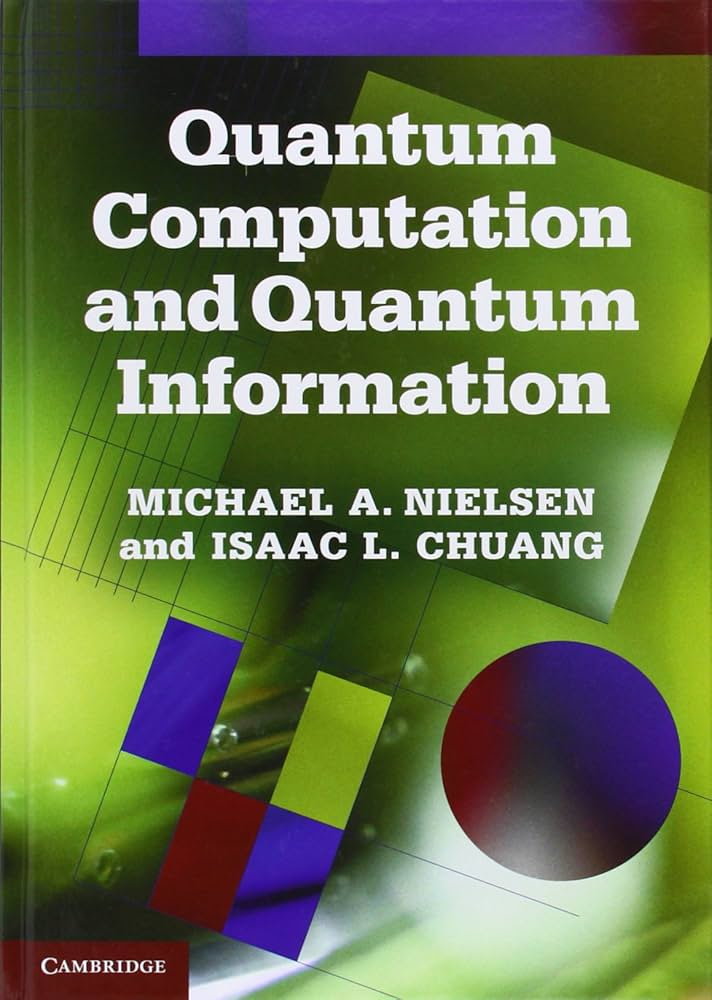
\includegraphics[width=.75\linewidth]{cover_nielsen_chuang.jpg}
      \caption{Section I and II}
      % \label{fig:sub2}
    \end{subfigure}
  \end{figure}
\end{frame}

\begin{frame}{The Double Slit Experiment}
  \begin{figure}[H]
    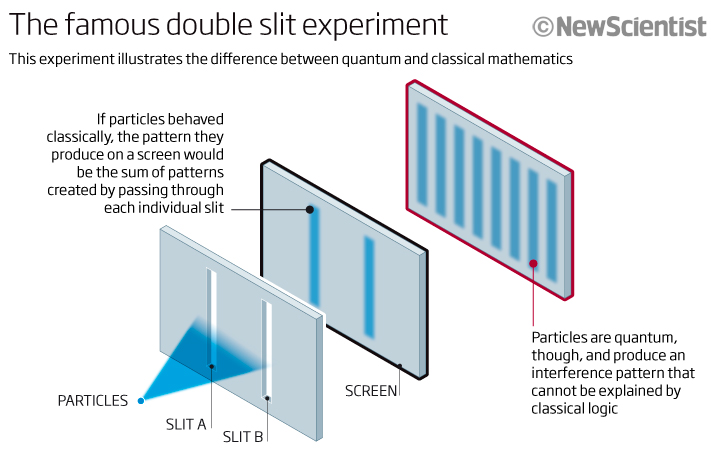
\includegraphics[scale=0.4]{electrons.jpg}
  \end{figure}
\end{frame}

\begin{frame}{Bits and qubits}
  \only<1-2>{
    In classical computing, data is represented through \emph{bits}. 
    
    A bit has two states: 0 or 1, true or false, on or off, etc. Physically, this is voltage on or off in a circuit.
  % }

  % \bigskip 

  % \only<2-2>{
    \pause The quantum analogue is a \emph{qubit}, and could physically be the spin of an electron (up or down) or the polarization of a photon (horizontal or vertical).

    A qubit has a \emph{continuum of states}.
  }
  \only<3-3>{
    A classical computer with \(m\) bits has \(2^m\) states.

    We can view each \emph{state as a basis vector for a \(2^m\)-dimensional vector space}, and \emph{each computation as a \(2^m \times 2^m \) matrix} acting on the state.

    A program is the composition of all the matrices describing the computations.
  }
  \only<4-4>{
    Suppose we have two bits \(x_1\) and \(x_2\). Our \emph{computational basis states} are 
    \begin{align*}
    \scalemath{0.75}{
      \ket{00} = \begin{pmatrix}1 \\ 0 \\ 0 \\ 0\end{pmatrix}, 
      \ket{01} = \begin{pmatrix}0\\1\\0\\0\end{pmatrix},
      \ket{10} = \begin{pmatrix}0\\0\\1\\0\end{pmatrix},
      \ket{11} = \begin{pmatrix}0\\0\\0\\1\end{pmatrix}.
    }
    \end{align*}
    The operation \(x_2 \mapsto x_1 \) (e.g. \(\ket{10} \mapsto \ket{11}\)) is described by 
    \begin{align*}
      \begin{pmatrix}
        1 & 1 & 0 & 0\\
        0 & 0 & 0 & 0\\
        0 & 0 & 0 & 0 \\
        0 & 0 & 1 & 1   
      \end{pmatrix}
    \end{align*}
  }
  \only<5>{
    If now our operation is 
    \begin{align*}
      \begin{cases}
        x_2 \mapsto x_1 & \text{with probability}\,\frac{1}{2}\\
        x_2 \mapsto x_2 \,\,(\text{do nothing}) & \text{with probability}\,\frac{1}{2}
      \end{cases}
    \end{align*}
    we have a corresponding \emph{stochastic matrix} 
    \begin{align*}
      \scalemath{0.75}{
      \begin{pmatrix}
        1 & \frac{1}{2} & 0 & 0 \\
        0 & \frac{1}{2} & 0 & 0 \\
        0 & 0 & \frac{1}{2} & 0 \\
        0 & 0 & \frac{1}{2} & 1
      \end{pmatrix}
      }
    \end{align*}
    \emph{Vectors in the state space are now probability distributions}, e.g. \[U \ket{10} = \frac{1}{2}(\ket{10} + \ket{11})\] and the computer has an equal chance of being in either \(\ket{10}\) or \(\ket{11}\).
  }
  \only<6>{
    A qubit has states in \(\C^2\), such as the \emph{computational basis states}
    \begin{align*}
      \ket{0} \coloneqq \begin{pmatrix}
        1 \\ 0
      \end{pmatrix}, 
      \qquad 
      \ket{1} \coloneqq \begin{pmatrix}
        0 \\ 1
      \end{pmatrix}
    \end{align*}
    Quantum particles can also be in complex linear combinations (\emph{superpositions}) of states: 
    \begin{align*}
      \ket{\psi} = \alpha \ket{0} + \beta \ket{1}.
    \end{align*} 
    \(\alpha\) and \(\beta\) are known as the \emph{amplitudes}. As they are complex, they can interfere \emph{constructively and destructively}.
  }
  \only<7>{
    If we measure a qubit, we either measure 0 or 1; \emph{nothing else!} 
    
    If the qubit has the state \(\ket{\psi} = \alpha \ket{0} + \beta \ket{1}\), then 
    \begin{align*}
      \mathbb{P}(\text{Measuring 0}) &= \abs{\alpha}^2 \\
      \mathbb{P}(\text{Measuring 1}) &= \abs{\beta}^2 \\
      \text{Total Probability} &= \abs{\alpha}^2 + \abs{\beta}^2 = 1 = \norm{\psi}^2
    \end{align*} 
    The state of a qubit is unobservable; when measuring, we only get information about the state.
  }
  \only<8>{
    We describe operations on our qubits through matrices acting on our state.

    We need our matrices to preserve total probability. Computations are therefore described by \emph{unitary matrices}, as these preserve the inner product.

    Unitary matrices are invertible, which is interpreted as \emph{reversible processes} and they \emph{cannot create or destroy information}.
  }
\end{frame}
\begin{frame}{Some example of unitary operators}
  \only<1>{
    \emph{Pauli matrices:}
    \begin{align*}
      % \scalemath{0.75}{
        \sigma_x = \begin{pmatrix}
          0 & 1 \\
          1 & 0 
        \end{pmatrix},
        \sigma_y = \begin{pmatrix}
          0 & -i \\
          i & 0
        \end{pmatrix}, 
        \sigma_z = \begin{pmatrix}
          1 & 0 \\
          0 & -1
        \end{pmatrix} 
      % }
    \end{align*}
    \(\sigma_x\) acts as a classical NOT-gate, e.g \(\sigma_x \ket{0} = \ket{1}\), \(\sigma_x \ket{1} = \ket{0}\).

    \(\sigma_y\) and \(\sigma_z\) are more quantum as they introduce phase changes:  
    \begin{align*}
      \sigma_y \ket{0} = i \ket{1}, \, \sigma_y \ket{1} = -i \ket{0} \\
      \sigma_z \ket{0} = \ket{0}, \, \sigma_z \ket{1} = -\ket{1} 
    \end{align*}
  }
  \only<2>{
    \emph{Hadamard matrix:} 
    \begin{align*}
      H = \frac{1}{\sqrt{2}} \begin{pmatrix}
        1 & 1 \\
        1 & -1
      \end{pmatrix}
    \end{align*}
    Maps \(\ket{0}\) and \(\ket{1}\) to superpositions of the two where each state is equally likely (\emph{uniform superposition}); 
    \begin{align*}
      H \ket{0} &= \frac{1}{\sqrt{2}} (\ket{0} + \ket{1}) \eqqcolon \ket{+} \\  
      H \ket{1} &= \frac{1}{\sqrt{2}} (\ket{0} - \ket{1}) \eqqcolon \ket{-}
    \end{align*}
    \(\ket{\pm}\) are the eigenvectors of \(\sigma_x\) and are called the \(X\)-basis. 
    
    % % As \(H = H^{-1}\) and \(
    % %   \sigma_x = H \sigma_z H
    % % \),
    % \(H\) acts as a basis change with \(\sigma_x \leftrightarrow \sigma_z\).
  }
\end{frame}

\begin{frame}{Multiple qubits}
  If we have \(N\) qubits, their states live in \((\C^2)^{\otimes N}\). 
  
  Our \(N\)-qubit basis vectors are the tensor products of single qubit each basis vector; e.g.
  \begin{align*}
    \ket{10} \coloneqq \scalemath{0.75}{
      \begin{pmatrix}
        0 \\ 0 \\ 1 \\ 0
      \end{pmatrix}
    }
    = \ket{1} \otimes \ket{0} 
    \eqqcolon \ket{1, 0}
  \end{align*}
  As 
  \begin{align*}
    \scalemath{0.75}{
      \begin{pmatrix}
        u_0 \\ u_1
      \end{pmatrix}
      \otimes  
      \begin{pmatrix}
        v_0 \\ v_1
      \end{pmatrix}
      =
      \begin{pmatrix}
        u_0 v_0 \\
        u_0 v_1 \\
        u_1 v_0 \\
        u_1 v_1
      \end{pmatrix}
    }
  \end{align*}
  the amplitudes of the joint state \(\ket{u,v}\) are the products of the amplitudes of \(\ket{0}\) and \(\ket{1}\).
\end{frame}

\begin{frame}
  Quantum computers can be faster than classical computers due to 
  \begin{itemize}
    \item \emph{Parallelism} -- e.g. qubits being in a superposition of states
    \item \emph{Interference} -- amplitudes are complex, so can combine constructively and destructively
  \end{itemize}
\end{frame}

\begin{frame}{Deutsch's algorithm}
  \only<1>{
    Let \(f \colon \set{0, 1} \to \set{0,1}\). Does \(f(0) = f(1)\)?

    Classically, can determine through two \emph{queries}: calculating \(f(0)\) and \(f(1)\) separately.
  }
  \only<2>{
    Consider a two qubit computer in state \(\ket{x, y}\). Define the unitary map 
    \begin{align*}
      U_{f} \ket{x, y} = \ket{x, y \oplus f(x)}
    \end{align*}
    where \(\oplus\) is addition mod 2.   
    
    If \(x\) is in the uniform superposition \(\ket{+} = \frac{1}{\sqrt{2}} (\ket{0} + \ket{1})\) and \(y\) in the state \(\ket{0}\), then  
    \begin{align*}
      U_{f} \ket{ + , \ket{0} }
      =
      \frac{1}{\sqrt{2}} \left(
        \ket{0, f(0)} + \ket{1, f(1)}
      \right)
    \end{align*}
    We have found information about \(f(0)\) and \(f(1)\) with only one computation; this is \emph{parallelism}.
  }
  \only<3>{
    We can improve this by using \emph{interference} to be better than classical computation. Notice that 
    \begin{align*}
      U_{f}\ket{x, y} = \ket{x} \otimes \sigma_{x}^{f(x)}\ket{y}
    \end{align*}
    \(\ket{-} = \frac{1}{\sqrt{2}}(\ket{0} - \ket{1})\) is an \emph{eigenvector for \(\sigma_{x}\)} with eigenvalue \(-1\), so 
    \begin{align*}
      U_{f} \ket{x, -} = (-1)^{f(x)} \ket{x, -}.
    \end{align*}
    Now preparing \(x\) in the state \(\ket{+}\) gives 
    \begin{align*}
      U_{f} \ket{+, -} 
      &= \frac{(-1)^{f(0)}\ket{0} + (-1)^{f(1)}\ket{1}}{\sqrt{2}} \otimes \ket{-} \\
      &\equiv \frac{\ket{0} + (-1)^{f(0) \oplus f(1)} \ket{1}}{\sqrt{2}} \otimes \ket{-}.
    \end{align*}
    If we now measure \(x\) as \(\ket{+}\) then \(f(0) = f(1)\).
  }
  \only<4>{
    This is known as \emph{phase kickback}: we prepare our `output qubit' \(y\) to be an eigenvector whose eigenvalue affects the phase of the `input qubit'.

    \bigskip

    By then measuring the `input' qubit \(x\) and not caring about the `output' qubit \(y\), we learn about \(f\).
  }
  \only<5>{
    Now consider \(f \colon \set{0,1}^{n} \to \set{0,1}\). We use a \((n+1)\)-qubit computer in the state \(\ket{\vec{x}, y}\) where \(\vec{x} \in \set{0,1}^n\).

    Consider again 
    \begin{align*}
      U_{f}\ket{\vec{x}, y} = \ket{\vec{x}, y \oplus f(\vec{x})} = \ket{\vec{x}} \otimes \sigma_{x}^{f(x)}\ket{y}.
    \end{align*}
    Let's try phase kickback again. Prepare the input qubits \(\vec{x}\) in a uniform superposition 
    \begin{align*}
      \frac{1}{\sqrt{2^n}} \sum_{\vec{x}} \ket{\vec{x}} 
      % = \ket{+}^{\otimes n}
    \end{align*}
    and the output qubit \(y\) in \(\ket{-}\) to get 
    \begin{align*}
      U_{f}\frac{1}{\sqrt{2^n}}\sum_{\vec{x}}\ket{\vec{x}, -} = \left(
        \frac{1}{\sqrt{2^n}} \sum_{\vec{x}} (-1)^{f(\vec{x})} \ket{\vec{x}}
      \right)
      \otimes \ket{-}.
    \end{align*}
  }
  \only<6>{
    The state 
    \begin{align*}
      \ket{\psi} 
      =
      \frac{1}{\sqrt{2^n}} \sum_{\vec{x}} (-1)^{f(\vec{x})} \ket{\vec{x}}
    \end{align*}
    again contains the values of \(f(\vec{x})\) in the phases of \(\vec{x}\)'s amplitudes.

    Questions:
    \begin{enumerate}
      \item What basis should we measure \(\ket{\psi}\) in?
      \item What can we learn when measuring \(\ket{\psi}\) about \(f\)?
    \end{enumerate}
  }
    % Deutsch-Jozsa, quantum fourier transformation
    
    % Simon's problem 

    % Shor's algorithm

    % Hidden subgroup problem


  %   Store \(x\) in a first qubit. 

  %   What does it mean to query a qubit \(f(x)\) in a quantum algorithm?

  %   If we set a second qubit \(y = f(x)\) as in the classical case, this destroys the information in \(y\) before.

  %   Instead, query \(f(x)\) reversibly by flipping \(y\) if \(f(x)\) is true:
  %   \begin{align*}
  %     U_{f}\ket{x, y} = \ket{x, y \oplus f(x)}
  %   \end{align*}
  %   Prepare \(x\) in the state \(\ket{+} = \frac{1}{\sqrt{2}} (\ket{0} + \ket{1})\) and \(y\) in the state \(\ket{0}\). Then 
  %   \begin{align*}
  %     U_{f}(\ket{+, 0}) = \frac{1}{\sqrt{2}}\Big(\ket{0, f(0)} + \ket{1, f(1)}\Big).
  %   \end{align*}
  % }
  % \only<3>{
  %   \(U_{f}(\ket{+, 0}) = \frac{1}{\sqrt{2}}\Big(\ket{0, f(0)} + \ket{1, f(1)}\Big)\) isn't that useful: measuring \(x\) gives us \(\ket{0,f(0)}\) and \(\ket{1, f(1)}\) with equal probability.
  % }
  % \only<4>{
  %   To improve, we use interference. Notice that 
  %   \begin{align*}
  %     U_{f} \ket{x, y} = \ket{x} \otimes \sigma_x^{f(x)} \ket{y}.
  %   \end{align*}
  %   Prepare \(y\) in the eigenvector of \(\sigma_x\) \(\ket{-} = \frac{1}{\sqrt{2}}(\ket{0} - \ket{1})\). This has eigenvalue \(-1\), so \(
  %     U_{f} \ket{x, -} = (-1)^{f(x)} \ket{x, -}
  %   \). Preparing \(x\) in \(\ket{+}\) gives 
  %   \begin{align*}
  %     U_{f} \ket{+, -} 
  %     = \frac{1}{\sqrt{2}} \Big((-1)^{f(0)}\ket{0} + (-1)^{f(1)} \ket{1}\Big) \otimes \ket{-} 
  %     \equiv 
  %     \frac{1}{\sqrt{2}} \Big(
  %       \ket{0} + (-1)^{f(0) \otimes f(1)} \ket{1}
  %     \Big)
  %   \end{align*}
  
  % If we observe our qubit and get \(\ket{+}\) then \(f(0) = f(1)\). 
  
  % If we observe our qubit and get \(\ket{-}\) then \(f(0) \neq f(1)\).
  % }
\end{frame}

\begin{frame}{The Quantum Fourier Transform}
  \emph{Discrete Fourier transform:} For \(x_0, \cdots, x_{N-1} \in \C\),
  \begin{align*}
    x_{j} \mapsto y_{j} = \frac{1}{\sqrt{N}}\sum_{k=0}^{N-1} e^{\frac{2\pi i j k}{N}} x_{k}
  \end{align*} 
  \emph{Quantum Fourier transform:} Defined by mapping the computational basis states 
  \begin{align*}
    \ket{j} 
    =
    \frac{1}{\sqrt{N}}
    \sum_{k=0}^{N-1} 
    e^{\frac{2\pi i j k}{N}}\ket{k}
  \end{align*}
  where \(0 \leq j \leq N-1\).
\end{frame}

\begin{frame}{QFT on \(\Z_{2}^{n}\)}
  Going back to \(\Z_{2}^{n}\), let \(\ket{\phi} = \sum_{\vec{x}}a_{x} \ket{x}\). We want to describe \(a_x\) as a linear combination of basis vectors oscillating at specific frequencies.

  Each frequency \(\vec{k} \in \Z_{2}^{n}\) has the basis function \((-1)^{\vec{k} \cdot \vec{x}}\) and basis state 
  \begin{align*}
    \ket{\vec{k}}
    =
    \frac{1}{\sqrt{2^n}} \sum_{\vec{x}}(-1)^{\vec{k} \cdot \vec{x}} \ket{x}
  \end{align*}
  giving us that 
  \begin{align*}
    \ket{\phi} 
    =
    \sum_{\vec{k}} \tilde{a}_{\vec{k}} \ket{k}, 
    \qquad
    \tilde{a}_{\vec{k}}
    =
    \frac{1}{\sqrt{2^n}}
    \sum_{\ket{x}}
    (-1)^{\vec{k} \cdot \vec{x}} a_{\vec{x}}
  \end{align*}
  This is \emph{equivalent to applying \(H^{\otimes n}\)}.
\end{frame}
\begin{frame}
  For our state \begin{align*}
    \ket{\psi} 
    =
    \frac{1}{\sqrt{2^n}} \sum_{\vec{x}} (-1)^{f(\vec{x})} \ket{\vec{x}}
  \end{align*}
  We apply the QFT \(H^{\otimes n}\) to \(\ket{\psi, 1}\) to get the frequency bits \(k_1 k_2 \cdots k_n\) written in the computational basis.

  Measuring a given \(\vec{k}\) has the probability 
  \begin{align*}
    \mathbb{P}(\vec{k})
    =
    \abs{\tilde{a}_{\vec{k}}}^2 
    =
    \abs{
      \frac{1}{2^n}
      \sum_{\vec{x}} (-1)^{\vec{k} \cdot \vec{x} + f(\vec{x})}
    }^2
  \end{align*}
  If \(n=1\), we have the Deutsch problem.  We have two frequencies \(k=0\) and \(k=1\).

  If \(f(0) = f(1)\) then \(\mathbb{P}(0) = 1\), \(\mathbb{P}(1) = 0\).

  If \(f(0) \neq f(1)\) then \(\mathbb{P}(0) = 0\), \(\mathbb{P}(1) = 1\).
\end{frame}

\begin{frame}{The Deutsch-Jozsa Problem}
  For \(f \colon \set{0,1}^n \to \set{0,1}\) suppose either is true: 
  \begin{enumerate}
    \item \(f\) is constant
    \item \(f\) is balanced: \(f(\vec{x}) = 0\) for half of all \(\vec{x}\), \(f(\vec{x}) = 1\) for the other half.
  \end{enumerate}
  Which is true?
\end{frame}
\begin{frame}
  The probability for observing the frequency of \((0, 0, \cdots, 0)\) is now encoded in
  \begin{align*}
    \tilde{a}_{\vec{0}}
    =
    \frac{1}{2^n} 
    \sum_{\vec{x}}(-1)^{f(\vec{x})}
  \end{align*}
  If \(f\) is constant, this is \( \pm 1\). If \(f\) is balanced, this is \(0\), so 
  \begin{align*}
    \mathbb{P}(\vec{0}) 
    =
    \abs{\tilde{a}_{\vec{0}}}^2
    =
    \begin{cases}
      0 & \text{if \(f\) balanced},\\
      1 & \text{if \(f\) constant}
    \end{cases}
  \end{align*}
  so we answer the Deutsch-Jozsa problem with just one observation.
\end{frame}

\begin{frame}{The plan for next time}
  \begin{itemize}
    \item Simon's problem 
    \item Shor's algorithm 
    \item Generalising our problems: the hidden subspace problem
  \end{itemize}
\end{frame}

\maketitle 

\begin{frame}{What we saw last time}
  \only<1>{
    Quantum particles behave very differently to the world we are used to.

    \bigskip

    They are \emph{wave-like} -- constructive and destructive interference.

    \bigskip

    They are inherently \emph{probabilistic} -- repeated measurements of identically prepared system may give different observations.
  }
  \only<2>{
    A qubit is our quantum version of a bit.
    
    \bigskip

    Physically, could be spin up/down of an electron, horizontal/vertical polarisation of light, etc.
  }
  \only<3>{
    Mathematically, a qubit lives in \(\C^2\) with Euclidean norm, and states (vectors with norm 1) we can observe (in the \emph{computational basis}) are 
    \begin{align*}
      \ket{0} \coloneqq \begin{pmatrix}
        1 \\ 0
      \end{pmatrix}, 
      \quad 
      \ket{1} \coloneqq \begin{pmatrix}
        0 \\ 1
      \end{pmatrix}
    \end{align*}
  Qubits could be in \emph{superpositions} of these states, e.g. \( \ket{\psi} = \alpha \ket{0} + \beta \ket{1}\). 
  
  We \emph{can't observe \(\ket{\psi}\)}; instead, 
  \begin{align*}
    \mathbb{P}(\text{observing}\, 0) = \abs{\alpha}^2
    &\qquad 
    \mathbb{P}(\text{observing}\, 1) = \abs{\beta}^2 \\
    \mathbb{P}(\text{observing}) &= 1 = \norm{\ket{\psi}}^2
  \end{align*}
  \(N\) qubits live in \((\C^2)^{\otimes N}\).
  }

  \only<4>{
    Abusing quantum properties can give us probabilistic methods to work out problems with less computations. 
    
    A method that we saw before for slightly constructed problems:
    \begin{enumerate}
      \item Set up input and output qubits to be in convenient states
      \item Apply a unitary operator to cleverly separate information about a given function into the input qubits
      \item Change our basis into one which is more convenient to work in 
      \item Take measurements to get information of our function to solve a question
    \end{enumerate}
  }
  \only<5>{
    The \emph{quantum Fourier transform} takes us to the computational basis to one where state amplitudes are in frequencies:
    \begin{align*}
      \ket{j} 
      \mapsto 
      \frac{1}{\sqrt{N}}
      \sum_{k=0}^{N-1} 
      e^{\frac{2\pi i j k}{N}}\ket{k}
    \end{align*}
      This proved useful to us previously as \emph{measuring certain frequencies could give us probabilistic methods} to give us \emph{information about a given function} based on what we can measure
      % On \(\Z_{2}^{N}\), each frequency \(\vec{k} \in \Z_{2}^{N}\) has the basis function \((-1)^{\vec{k} \cdot \vec{x}}\) and basis state 
      % \begin{align*}
      %   \ket{\vec{k}}
      %   =
      %   \frac{1}{\sqrt{2^N}} \sum_{\vec{x}}(-1)^{\vec{k} \cdot \vec{x}} \ket{x}
      % \end{align*}
      
      % For \(\ket{\phi} = \sum_{\vec{x}}a_{x} \ket{x}\), the QFT gives us 
      % \begin{align*}
      %   \ket{\phi} 
      %   =
      %   \sum_{\vec{k}} \tilde{a}_{\vec{k}} \ket{k}, 
      %   \qquad
      %   \tilde{a}_{\vec{k}}
      %   =
      %   \frac{1}{\sqrt{2^N}}
      %   \sum_{\ket{x}}
      %   (-1)^{\vec{k} \cdot \vec{x}} a_{\vec{x}}
      % \end{align*}
  }
  
  % \only<4>{
  %     Abusing quantum properties can give us probabilistic methods to work out problems with less computations.
    
  %     E.g. the \emph{Deutsch-Jozsa problem}: for \(f \colon \set{0,1}^N \to \set{0,1}\) with either 
  %     \begin{itemize}
  %       \item \(f\) is constant 
  %       \item \(f\) is balanced; e.g. \(f(x) = 0\) for half of \(x\), \(f(x) = 1\) for the other half 
  %     \end{itemize}
  %     How do we know which is true?
  % }
  % \only<5>{
  %   Trick: move into a basis where information is more easily accessible.
  
  % The \emph{quantum Fourier transform} takes us to the computational basis to one where state amplitudes are in frequencies:
  % \begin{align*}
  %   \ket{j} 
  %   \mapsto 
  %   \frac{1}{\sqrt{N}}
  %   \sum_{k=0}^{N-1} 
  %   e^{\frac{2\pi i j k}{N}}\ket{k}
  % \end{align*}
  %   On \(\Z_{2}^{N}\), each frequency \(\vec{k} \in \Z_{2}^{N}\) has the basis function \((-1)^{\vec{k} \cdot \vec{x}}\) and basis state 
  %   \begin{align*}
  %     \ket{\vec{k}}
  %     =
  %     \frac{1}{\sqrt{2^N}} \sum_{\vec{x}}(-1)^{\vec{k} \cdot \vec{x}} \ket{x}
  %   \end{align*}
    
  %   For \(\ket{\phi} = \sum_{\vec{x}}a_{x} \ket{x}\), the QFT gives us 
  %   \begin{align*}
  %     \ket{\phi} 
  %     =
  %     \sum_{\vec{k}} \tilde{a}_{\vec{k}} \ket{k}, 
  %     \qquad
  %     \tilde{a}_{\vec{k}}
  %     =
  %     \frac{1}{\sqrt{2^N}}
  %     \sum_{\ket{x}}
  %     (-1)^{\vec{k} \cdot \vec{x}} a_{\vec{x}}
  %   \end{align*}
  % }
  % \only<6>{
  %   Solving Deutsch-Jozsa:
  %   \begin{enumerate}
  %     \item Prepare \(x\) input qubits in the uniform superposition \(\frac{1}{\sqrt{2^N}} \sum_{\vec{x}}\ket{x}\) and an output qubit \(y\) in \(\ket{-} \coloneqq \frac{1}{\sqrt{2}}(\ket{0} - \ket{1})\).
  %     \item Apply the unitary operator \(U_{f} \ket{x, y} = \ket{x} \otimes \sigma_{x}^{f(x)}\ket{y}\) to our qubits so we are in the state \begin{align*}
  %         U_{f}\frac{1}{\sqrt{2^N}}\sum_{\vec{x}}\ket{\vec{x}, -} = \left(
  %         \frac{1}{\sqrt{2^N}} \sum_{\vec{x}} (-1)^{f(\vec{x})} \ket{\vec{x}}
  %       \right)
  %       \otimes \ket{-}
  %       \end{align*}
  %     Now our \(x\) amplitudes are in terms of \(f(x)\).
  %   \end{enumerate}
  % }
  % \only<7>{
  %   \begin{enumerate}
  %     \setcounter{enumi}{2}
  %     \item Apply QFT to get frequency bits in the computational basis. Measuring a given \(\vec{k}\) has the probability 
  %     \begin{align*}
  %       \mathbb{P}(\vec{k})
  %       =
  %       \abs{\tilde{a}_{\vec{k}}}^2 
  %       =
  %       \abs{
  %         \frac{1}{2^n}
  %         \sum_{\vec{x}} (-1)^{\vec{k} \cdot \vec{x} + f(\vec{x})}
  %       }^2
  %     \end{align*}
  %     \item Measuring the 0 frequency gives us that \begin{align*}
  %       \mathbb{P}(\vec{0}) 
  %       =
  %       \abs{\tilde{a}_{\vec{0}}}^2
  %       =
  %       \begin{cases}
  %         0 & \text{if \(f\) balanced},\\
  %         1 & \text{if \(f\) constant}
  %       \end{cases}
  %     \end{align*}
  %   \end{enumerate}
  % }
\end{frame}

\begin{frame}{Simon's problem}
  \begin{block}{Simon's Problem}
    Let \(f \colon \set{0,1}^{n} \to \set{0,1}^n\) such that 
    \begin{align*}
      f(x) = f(x^\prime) 
      \iff 
      x^\prime = x \oplus r
    \end{align*}
    for some fixed \(r\). How many computations on \(f\) to determine \(r\)?
  \end{block}
\end{frame}
\begin{frame}
  \begin{enumerate}
    \item Define \(U_{f} \ket{x, y} = \ket{x, y \oplus f(x)}\).
    \item Prepare the input qubits \(x\) in a uniform superposition, prepare the output qubits \(y\) in \(\ket{0}\).
    \item \(U_{f}\frac{1}{\sqrt{2^n}}\sum_{x}\ket{x, 0} = \frac{1}{\sqrt{2^n}} \sum_{x} \ket{x, f(x)}\).
    \item Observe \(f(x)\) to be some \(f_0\). Our state collapses to the \(x\) with \(f(x) = f_0\), \(\ket{\psi, f_0}\) where 
    for some \(x_0\) \begin{align*}
      \ket{\psi} = \frac{1}{\sqrt{2}} (\ket{x_0} + \ket{x_0 \oplus r})
    \end{align*}
  \end{enumerate}
\end{frame}
\begin{frame}
  \begin{enumerate}
    \setcounter{enumi}{4}
    \item Measure \(\psi\) in Fourier basis. We observe a given frequency \(k\) with chance \begin{align*}
      \mathbb{P}(k) =
      \begin{cases}
          \frac{1}{2^{n-1}} & \text{if \(k\) and \(r\) are orthogonal} \\
          0 & \text{otherwise}
      \end{cases}
    \end{align*}
    \item The vectors perpendicular to \(r\) form a \((n-1)\)-dimensional subspace, so observe enough \(k\)'s that span this subspace. This happens by computing \(f\) roughly \(n\) times.
  \end{enumerate}
\end{frame}

\begin{frame}{Shor's factoring algorithm}
  In the first talk, we saw that RSA is a cryptosystem we have faith in because to break it, you need to be able to factor large numbers.

  \bigskip

  Factoring for classical computers is difficult and takes a long time. For quantum computers, it is a lot easier.
\end{frame}

\begin{frame}
  Suppose we want to find a non-trivial factor of \(N\).
  \begin{enumerate}
    \item If \(N\) even, return \(2\).
    \item Use classical algorithm to determine if \(N = a^b\) for \(a \geq 1\), \(b \geq 2\). If so, return \(a\).
    \item Guess \(x \in \set{3, \cdots, N-1}\) to be a factor. If \(\mathrm{gcd}(x, N) > 1\), return \(\mathrm{gcd}(x, N)\).
    \item Use quantum algorithm to find the smallest \(r\) such that \(x^{r} \equiv 1 \mod N\).
    \item If \(r\) even and \(x^{\frac{r}{2}} \not\equiv -1 \mod N\), check if \(\mathrm{gcd}(x^{\frac{r}{2}}-1, N)\) or \(\mathrm{gcd}(x^{\frac{r}{2}}+1, N)\) is a factor.
    \item If none of the above was successful, the algorithm fails.
  \end{enumerate}
\end{frame}
\begin{frame}{The quantum order finding algorithm}
  With `enough' input qubits \(t\) and output qubits:
  \begin{enumerate}
    \item Prepare input qubits in a uniform superposition \(\frac{1}{\sqrt{2^t}}\sum_{j=0}^{2^t - 1}\ket{j, 1}\)
    \item Apply unitary operator \(U \ket{j, k} = \ket{j, x^j \mod N}\) for our guess of a factor \(x\)
    \item \(\ket{1}\) can be written as a sum of eigenstates \(u_{s}\) of \(U\) with Fourier coefficients, so applying inverse Fourier transform gives us the state \begin{align*}
      \frac{1}{\sqrt{r}} \sum_{s = 0}^{r-1} \ket{\frac{s}{r}, u_{s}}.
    \end{align*}
    \item Take measurement to get \(\frac{s}{r}\), apply the \emph{continued fractions algorithm} to get \(r\).
  \end{enumerate}
\end{frame}
\begin{frame}
  The factoring problem falls into the class of \emph{bounded-error quantum polynomial time} (BQP) problems.

  \bigskip 

  These problems can be solved in \emph{polynomial-time} by quantum algorithms which \emph{give the correct answer at least \(\frac{2}{3}\) of the time}.
\end{frame}


\begin{frame}
  Order finding is a special case of the period finding problem, and we can express it as the following:

  \begin{block}{Order finding as periodicity}
    Fix \(a\) such that \(a^r \equiv 1 \mod N\) and \(f \colon \Z \to \set{a^j \colon j \in \Z_{r}}\) with 
    \begin{align*}
      f(x) = a^x, \qquad f(x+r) = f(x)
    \end{align*}

    How do we find \(r\)?
  \end{block}
  This is the same sort of problem as we've seen previously.
\end{frame}
% \begin{frame}
%   For the period-finding problem, consider \(f \colon \Z_{M} \to S\) for a sufficiently large \(M\) such that 
%   \begin{align*} 
%     f(x) = f(x^\prime) \iff x \equiv x^\prime \mod r. 
%   \end{align*}
%   \vspace{-1cm}
%   \begin{enumerate}
%     \item Prepare qubits \(\ket{x, f(x)}\) where \(x\) are in a uniform superposition.
%     \item Measure \(f(x)\) as \(f_0\) to end up in the state \(\ket{\psi, f_0}\) where \(\psi\) is in the uniform superposition of \(x\) where \(f(x) = f_0\), so \begin{align*}
%       \ket{\psi} 
%       =
%       \sqrt{\frac{r}{M}} \sum_{x \equiv x_0 \mod r } \ket{x}
%     \end{align*}
%     \item Convert to Fourier basis and get that the probability to observe a frequency \(k\) is \begin{align*}
%       \mathbb{P}(k) 
%       =
%       \begin{cases*}
%         \frac{1}{r} & \text{if \(k\) is a multiple of \(\frac{M}{r}\)} \\
%         0 & \text{otherwise}
%       \end{cases*}
%     \end{align*}
%   \end{enumerate}
% \end{frame}
\begin{frame}{Diffie-Hellmann}
  As we saw previously, Diffie-Hellmann key exchange is a way to share symmetric public keys securely in public channels, and can be attacked by quantum computers via the \emph{discrete logarithm problem}:

  \begin{block}{Discrete Logarithm Problem}
    Fix \(a, N \in \Z\) and let \(r\) be smallest number with \(a^r \equiv  1 \mod N\). Define \(f \colon \Z_{r} \times \Z_{r} \to \set{a^{j} \colon j \in \Z_{r}}\), 
    \begin{align*}
      f(x_1, x_2) = a^{sx_{1} + x_{2}}
    \end{align*}
    which has the period \((l, -sl)\) for some choice of \(l\). What is \(s\)?
  \end{block}
\end{frame}

\begin{frame}{The Hidden Subgroup Problem}
  \begin{block}{Hidden Subspace Problem}
    Let \(G\) be a group, \(f \colon G \to S\) a function such that there is a subgroup \(H \subseteq G\) with 
    \begin{align*}
      f(x) = f(x^\prime) 
      \iff 
      x^\prime = xh
      \,\,
      \text{for some} 
      \,\,
      h \in H.
    \end{align*}

    What is \(H\)?
  \end{block}
\end{frame}
\begin{frame}{Solving HSP for Finite Abelian Groups}
  Quantum computers can easily solve the hidden subgroup problem for finite Abelian groups:
  \begin{itemize}
    \item Prepare qubits in uniform superposition \(\frac{1}{\sqrt{\abs{G}}} \sum_{g \in G} \ket{g, f(g)}\).
    \item Convert \(\ket{f(g)}\) into Fourier basis: \begin{align*}
      \ket{f(g)} = \frac{1}{\sqrt{\abs{G}}}\sum_{j = 0}^{\abs{G} - 1} \exp(\frac{2\pi i j g}{\abs{G}}) \ket{\hat{f}(j)}
    \end{align*} which, as \(f\) is constant and different on each coset of \(G\), has nearly zero amplitude for all values of \(j\) except those satisfying \begin{align*}
      \sum_{h \in H} \exp(\frac{-2 \pi i j h}{\abs{G}}) = \abs{H}
    \end{align*}
  \end{itemize}
\end{frame}
\begin{frame}
  \begin{itemize}
    \item As \(G\) is finite Abelian, there exists primes \(p_1, \cdots, p_N\) such that \(G \cong Z_{p_1} \times \cdots \times Z_{p_N}\), so for \(g_k \in Z_{p_k}\) we get \begin{align*}
      \exp(\frac{2\pi i j g}{\abs{G}})
      =
      \prod_{j=k}^{N} \exp(\frac{2 \pi i j^{\prime}_{k} g_{k} }{p_k})
    \end{align*} 
    \item An algorithm known as \emph{phase estimation} gets us \(j_{k}^{\prime}\), which lets us find the \(j\) for which the amplitudes of \(\ket{\hat{f}(j)}\) are not nearly 0, which lets us find \(H\).
  \end{itemize}
\end{frame}
\begin{frame}{An interesting problem to look into}
  Things aren't as simple in the non-Abelian case -- this would take multiple talks by itself!

  A nice natural non-Abelian problem which can be formed as a Hidden Subgroup Problem is the \emph{graph isomorphism problem}:
  \begin{block}{Graph Isomorphism Problem}
    If \(G_1, G_2\) are two graphs, is there a permutation \(\pi\) on the edges with \(\pi(G_1) = G_2\)? I.e. are the graphs topologically equivalent? 
  \end{block}
  \begin{itemize}
      \item {``Quantum algorithms for algebraic problems" by A. Childs and W. van Dam} 
      \item {``The Nature of Computing" by C. Moore and S. Mertens, Ch 15.6}
  \end{itemize}
\end{frame}

% \begin{frame}{Norms}
%     \only<1, 2, 3>{
%     \begin{alertblock}{Norm}
%       A {\emph{norm}} on $V$ is a function $\norm{\cdot}: V \to \C$ such that for all $x, y \in V$ and $\lambda \in \C$,
%       \begin{enumerate}
%         \item $\norm{x + y} \leq \norm{x} + \norm{y}$,
%         \item $\norm{\lambda x} = \abs{\lambda}\norm{x}$,
%         \item $\norm{x} = 0$ if and only if $x = 0$
%       \end{enumerate}
%   \end{alertblock}
%     }
%     \only<2,3>{
%     It turns out that the function $\norm{\cdot} \coloneqq \sqrt{\ip{\cdot,\cdot}}$ is a norm, which we call the {\emph{norm induced by the inner product}}.
%
%     }
%     \only<3>{
%     It is the only type of norm that we'll be interested in!
%     }
%
% \end{frame}

% % % \begin{frame}[allowframebreaks]{References}

% % %   \nocite{*}
% % %   \bibliography{references}
% % %   \bibliographystyle{abbrv}

% % \end{frame}
\end{document}
